\documentclass[border=1pt]{standalone}
\usepackage[table]{xcolor}
\definecolor{dnvang}{HTML}{E5890A}
\definecolor{dnxanh}{HTML}{3A98B9}
\definecolor{dnxanhdam}{HTML}{006A90}
\definecolor{dndo}{HTML}{BB2649}
\def\mycolor{dnvang}
\def\mauphu{dnxanh}
\def\maudam{dnxanhdam}
\def\maunhan{dndo}
\usepackage[utf8]{vietnam}
\usepackage{tikz}
\usetikzlibrary{angles,quotes,intersections,fit}
\usetikzlibrary{calc,fadings,shadows,shadows.blur,shapes.geometric,positioning,backgrounds,decorations.pathmorphing,decorations,matrix}
\usepackage{graphicx}
\usepackage{tikz-3dplot,pgfplots}
\pgfplotsset{compat=1.15}
\usepgfplotslibrary{polar}
\usepackage{amsmath}
\usepackage{multicol,environ,etoolbox}
\usepackage{pifont,oplotsymbl,marvosym,fontawesome}
\usepackage{multido} % gói thêm dòng kẻ
\begin{document}
	%%=============AOPx=====================%%%
	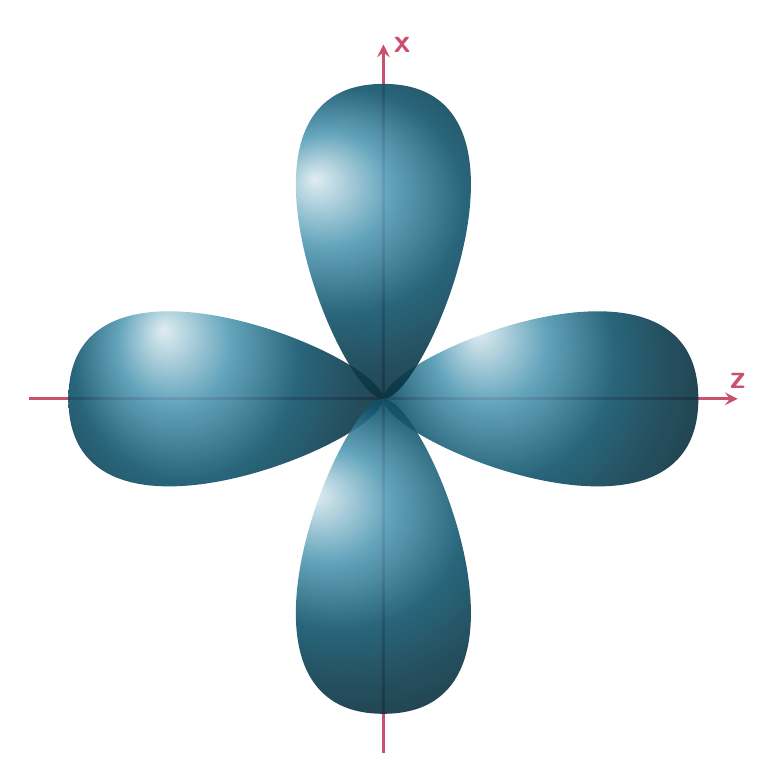
\begin{tikzpicture}[declare function={d=4cm;r=2.2cm;h=.5cm;}]
		\tikzstyle{linestyle} = [->,>=stealth,line width=1pt,\maunhan!80]
		\tikzstyle{myshapestyle} = [line width=1pt,ball color = \maudam!90,opacity=.90]
		\draw[linestyle] ({-d - h},0)--({d + h},0)node[above,font=\large\sffamily\bfseries]{ z};
		\draw[linestyle] (0,{-d - h})--(0,{d + h})node[right,font=\large\sffamily\bfseries]{ x};
		\path[myshapestyle] (-d,0)..controls +(90:r) and +(90:{.25*r})..(0,0)--
		(0,0)..controls +(-90:{.25*r}) and +(-90:r)..(-d,0);
		\path[myshapestyle] (d,0)..controls +(90:r) and +(90:{.25*r})..(0,0)--
		(0,0)..controls +(-90:{.25*r}) and +(-90:r)..(d,0);
		\path[myshapestyle] (0,0)..controls +(0:{.25*r}) and +(0:r)..(0,d)--
		(0,d)..controls +(180:r) and +(180:{.25*r})..(0,0);
		\path[myshapestyle] (0,-d)..controls +(180:r) and +(180:{.25*r})..(0,0)--
		(0,0)..controls +(0:{.25*r}) and +(0:r)..(0,-d);
	\end{tikzpicture}
%	%%%============= Sự xen phủ AO S-S =====================%%%
%	\begin{tikzpicture}[declare function={d=2cm;h=.05*d;},node font=\bfseries\sffamily\large]
%		\tikzstyle{linestyle} = [line width=2pt,\maunhan!80,->,>=stealth]
%		\tikzstyle{myshapestyle} = [line width=1pt,ball color = \maunhan!90,opacity=.65]
%		\draw[\maunhan,dashed,line width=1pt] ([xshift=-d]0,0)--([xshift=d]0,0);
%		\fill[myshapestyle] (0,0) circle (.75*d);
%	    \node at (1.5*d,0) (plus) {\color{\maunhan}+};
%		\draw[\maunhan,dashed,line width=1pt] ([xshift=-d]3*d,0)--([xshift=d]3*d,0);
%		\fill[myshapestyle] (3*d,0) circle (.75*d);
%		\draw[linestyle] (4.5*d,0)--(6*d,0);
%		\draw[\maunhan,dashed,line width=1pt] ([xshift=-1.5*d]8*d,0)--([xshift=1.5*d]8*d,0);
%		\fill[myshapestyle] (7.5*d,0) circle (.75*d);
%		\fill[myshapestyle] (8.5*d,0) circle (.75*d);
%		\node at ([shift={(-90:d)}]0,0) {AO s};
%		\node at ([shift={(-90:d)}]3*d,0) {AO s};
%		\node at ([shift={(-90:d)}]8.0*d,0) {Xen phủ trục s-s};
%	\end{tikzpicture}
%		%%%============= Sự xen phủ AO p-p =====================%%%
%	\begin{tikzpicture}[declare function={d=1.75cm;r=.55*d;h=0.125*d;},node font=\bfseries\sffamily]
%			\tikzstyle{linestyle} = [->,>=stealth,line width=1pt,\maunhan!80]
%			\tikzstyle{myshapestyle} = [line width=1pt,ball color = \maudam!90,opacity=.90]
%			\draw[line width=1pt,\maunhan!80] ([xshift=-1.1*d]0*d,0)--([xshift=1.1*d]0*d,0);
%			\path[myshapestyle] (-d,0)..controls +(90:r) and +(90:{.25*r})..(0,0)--
%			(0,0)..controls +(-90:{.25*r}) and +(-90:r)..(-d,0);
%			\path[myshapestyle] (d,0)..controls +(90:r) and +(90:{.25*r})..(0,0)--
%			(0,0)..controls +(-90:{.25*r}) and +(-90:r)..(d,0);
%			%%%==================================%%%
%			\draw[line width=1pt,\maunhan!80] ([xshift=-1.1*d]3*d,0)--([xshift=1.1*d]3*d,0);
%			\path[myshapestyle] (2*d,0)..controls +(90:r) and +(90:{.25*r})..(3*d,0)--
%			(3*d,0)..controls +(-90:{.25*r}) and +(-90:r)..(2*d,0);
%			\path[myshapestyle] (4*d,0)..controls +(90:r) and +(90:{.25*r})..(3*d,0)--
%			(3*d,0)..controls +(-90:{.25*r}) and +(-90:r)..(4*d,0);
%			%%%==================================%%%
%			\draw[line width=1pt,\maunhan!80] ([xshift=-2.05*d]7.875*d,0)--([xshift=2.05*d]7.875*d,0);
%			\path[myshapestyle] (6*d,0)..controls +(90:r) and +(90:{.25*r})..(7*d,0)--
%			(7*d,0)..controls +(-90:{.25*r}) and +(-90:r)..(6*d,0);
%			\path[myshapestyle] (8*d,0)..controls +(90:r) and +(90:{.25*r})..(7*d,0)--
%			(7*d,0)..controls +(-90:{.25*r}) and +(-90:r)..(8*d,0);
%			%%%==================================%%%
%			\path[myshapestyle] (7.75*d,0)..controls +(90:r) and +(90:{.25*r})..(8.75*d,0)--
%			(8.75*d,0)..controls +(-90:{.25*r}) and +(-90:r)..(7.75*d,0);
%			\path[myshapestyle] (9.75*d,0)..controls +(90:r) and +(90:{.25*r})..(8.75*d,0)--
%			(8.75*d,0)..controls +(-90:{.25*r}) and +(-90:r)..(9.75*d,0);
%			\draw[linestyle,line width=0.05*d] (4.5*d,0)--(5.5*d,0);
%			\node at (1.5*d,0) {+};
%			\node at ([shift=(-90:.55*d)]0*d,0) {AO p};
%			\node at ([shift=(-90:.55*d)]3*d,0) {AO p};
%			\node at ([shift=(-90:.55*d)]7.875*d,0) {Xen phủ trục p-p};
%	\end{tikzpicture}
	
	
\NewDocumentCommand{\AOs}{O{1.8}O{}O{}O{}}{%
		\ifblank{#2}{\def\tuychontwo{\maunhan}}{\def\tuychontwo{#2}}
		\ifblank{#3}{\def\tuychonthree{.80}}{\def\tuychonthree{#3}}
		\ifblank{#4}{\def\tuychonfour{densely dotted}}{\def\tuychonfour{#4}}
		\begin{tikzpicture}[declare function={d=#1cm;r=.65*d;h=0.125*d;R=.36*d;},node font=\bfseries\sffamily]
			\tikzstyle{linestyle} = [line width=0.015*d,\tuychontwo!80,\tuychonfour]
			\tikzstyle{myshapestyle}=[ball color = \tuychontwo,opacity=\tuychonthree]
			\draw[linestyle] ([xshift=-1.2*R]0*d,0)--([xshift=1.2*R]0*d,0);
			\fill[myshapestyle] (0*d,0) circle (R);
		\end{tikzpicture}
}
	


\NewDocumentCommand{\AOp}{O{1.8}O{}O{}O{}}{%
	\ifblank{#2}{\def\tuychontwo{\maunhan}}{\def\tuychontwo{#2}}
	\ifblank{#3}{\def\tuychonthree{.80}}{\def\tuychonthree{#3}}
	\ifblank{#4}{\def\tuychonfour{densely dotted}}{\def\tuychonfour{#4}}
	\begin{tikzpicture}[declare function={d=2cm;r=.65*d;h=0.125*d;R=.36*d;},node font=\bfseries\sffamily]
		\tikzstyle{linestyle} = [line width=0.015*d,\maunhan!80,\tuychonfour,>=stealth]
		\tikzstyle{myshapestyle} = [ball color = \tuychontwo,opacity=\tuychonthree]
		\draw[linestyle] ([xshift=-1.1*d]2*d,0)--([xshift=1.1*d]2*d,0);
		\path[myshapestyle] (1*d,0)..controls +(90:r) and +(90:{.25*r})..(2*d,0)--
		(2*d,0)..controls +(-90:{.25*r}) and +(-90:r)..(1*d,0);
		\path[myshapestyle] (3*d,0)..controls +(90:r) and +(90:{.25*r})..(2*d,0)--
		(2*d,0)..controls +(-90:{.25*r}) and +(-90:r)..(3*d,0);
	\end{tikzpicture}
}














%
%%%%=============Sự xen phủ bên=====================%%%
%
%\begin{tikzpicture}[declare function={d=3cm;r=.55*d;h=.125*d;R=.36*d;k=0.65*d;}]
%\tikzstyle{linestyle} = [line width=1pt,\maunhan!80,dashed]
%\tikzstyle{myshapestyle} = [line width=1pt,ball color = \maudam!90,opacity=.90]
%\tikzset{
%	pics/.cd,
%	AOsa/.style={code={
%		\draw[linestyle] ([xshift=-1.2*R]0*d,0)--([xshift=1.2*R]0*d,0);
%		\fill[myshapestyle] (0*d,0) circle (R);
%	}},
%	AOsb/.style={code={
%			\draw[linestyle] ([xshift=-1.2*R]0*d,0)--([xshift=1.2*R]0*d,0);
%			\fill[line width=1pt,ball color = \maunhan!90,opacity=.4] (0*d,0) circle (R);
%	}},
%	AOPa/.style={code={
%			\draw[linestyle] (0,{-d - h})--(0,{d + h});
%			\path[myshapestyle] (0,0)..controls +(0:{.25*r}) and +(0:r)..(0,d)--
%			(0,d)..controls +(180:r) and +(180:{.25*r})..(0,0);
%			\path[myshapestyle] (0,-d)..controls +(180:r) and +(180:{.25*r})..(0,0)--
%			(0,0)..controls +(0:{.25*r}) and +(0:r)..(0,-d);
%	}},
%	AOPb/.style={code={
%			\draw[linestyle] (0,{-d - h})--(0,{d + h});
%			\path[myshapestyle,ball color = \maunhan!90] (0,0)..controls +(0:{.25*r}) and +(0:r)..(0,d)--
%			(0,d)..controls +(180:r) and +(180:{.25*r})..(0,0);
%			\path[myshapestyle,ball color = \maunhan!90] (0,-d)..controls +(180:r) and +(180:{.25*r})..(0,0)--
%			(0,0)..controls +(0:{.25*r}) and +(0:r)..(0,-d);
%	}}}
%	\path (0,0) coordinate (A)
%	(1.5*k,0) coordinate (B)
%	(3*k,0) coordinate (C)
%	(6.4*k,0) coordinate (D)
%	($(D)+(0.75*r,0)$) coordinate (E)
%	;
%	\pic [local bounding box=AOPx] at (A) {AOsa};
%	\node(plus) at (1.5*k,0) {\color{\maunhan}\LARGE\bfseries\sffamily +};
%	\pic [local bounding box=AOPyt] at (C) {AOsb};
%	\pic [local bounding box=AOPy] at (C) {AOPa};
%	\pic [local bounding box=AOPz] at (D) {AOPa};
%	\path[draw,->,-latex,line width=.035*d,\maunhan!80] (AOPy)--(AOPz);
%	\pic [local bounding box=AOPt] at (E) {AOPa};
%	\node [font=\Large\bfseries\sffamily,shift={(-90:1.3*d)} ]at (A){AO p};
%	\node [font=\Large\bfseries\sffamily,shift={(-90:1.3*d)} ]at (C){AO p};
%	\node [font=\Large\bfseries\sffamily,shift={(-90:1.3*d)} ]at ($(D)!0.5!(E)$){Xen phủ bên p-p};
%\end{tikzpicture}

%\begin{tikzpicture}[declare function={d=3cm;r=.55*d;h=.125*d;R=.36*d;k=0.65*d;}]
%	\tikzstyle{linestyle} = [line width=1pt,\maunhan!80,dashed]
%	\tikzstyle{myshapestyle} = [line width=1pt,opacity=.90,ball color =\mauphu!90]
%	\tikzset{
%		pics/.cd,
%		AOs/.style args={#1/#2}{code={%
%				\if\relax\detokenize{#1}\relax
%				\def\ballcolor{red}
%				\else
%				\def\ballcolor{#1}
%				\fi,
%				\if\relax\detokenize{#2}\relax
%				\def\opacity{0.8}
%				\else
%				\def\opacity{#2}
%				\fi
%				\draw[linestyle] ([xshift=-1.2*R]0*d,0)--([xshift=1.2*R]0*d,0);
%				\fill[myshapestyle,ball color = \ballcolor,opacity=\opacity] (0*d,0) circle (R);
%		}},
%		AOp/.style={code={%
%				\draw[linestyle] (0,{-d - h})--(0,{d + h});
%				\path[myshapestyle] (0,0)..controls +(0:{.25*r}) and +(0:r)..(0,d)--
%				(0,d)..controls +(180:r) and +(180:{.25*r})..(0,0);
%				\path[myshapestyle] (0,-d)..controls +(180:r) and +(180:{.25*r})..(0,0)--
%				(0,0)..controls +(0:{.25*r}) and +(0:r)..(0,-d);
%		}}
%		}
%	\path (0,0) coordinate (A)
%	(1.5*k,0) coordinate (B)
%	(3*k,0) coordinate (C)
%	(6.4*k,0) coordinate (D)
%	($(D)+(0.75*r,0)$) coordinate (E)
%	;
%	\pic [local bounding box=AOsa] at (A) {AOs={red}/{}};
%	\node(plus) at (1.5*k,0) {\color{\maunhan}\LARGE\bfseries\sffamily +};
%	\pic [local bounding box=AOsb] at (C) {AOs={blue}/{}};
%	\pic [local bounding box=AOPy] at (C) {AOp};
%	\pic [local bounding box=AOPz] at (D) {AOp};
%	\path[draw,->,-latex,line width=.035*d,\maunhan!80] (AOPy)--(AOPz);
%	\pic [local bounding box=AOPt] at (E) {AOp};
%	\node [font=\Large\bfseries\sffamily,shift={(-90:1.3*d)} ]at (A){AO p};
%	\node [font=\Large\bfseries\sffamily,shift={(-90:1.3*d)} ]at (C){AO p};
%	\node [font=\Large\bfseries\sffamily,shift={(-90:1.3*d)} ]at ($(D)!0.5!(E)$){Xen phủ bên p-p};
%\end{tikzpicture}

























	
	%%%============= Sự xen phủ AO s-p =====================%%%
%	\begin{tikzpicture}[declare function={d=1.8cm;r=.65*d;h=0.125*d;R=.36*d;},node font=\bfseries\sffamily]
%		\tikzstyle{linestyle} = [line width=1pt,\maunhan]
%		\tikzstyle{myshapestyle} = [line width=1pt,ball color = \maudam!90,opacity=.80]
%%		\draw[linestyle] ([xshift=-1.2*R]0*d,0)--([xshift=1.2*R]0*d,0);
%%		\fill[myshapestyle,ball color=\maunhan] (0*d,0) circle (R);
%		%%===============================%%%
%%		\node at ({R+(d-R)/2},0) {+};
%		%%%==================================%%%
%		\draw[line width=1pt,\maunhan!80] ([xshift=-1.1*d]2*d,0)--([xshift=1.1*d]2*d,0);
%%		\draw[line width=1pt,\maunhan!80] ([xshift=-.2*R]4.64*d,0)--([xshift=.2*R]7.22*d,0);
%		\path[myshapestyle] (1*d,0)..controls +(90:r) and +(90:{.25*r})..(2*d,0)--
%		(2*d,0)..controls +(-90:{.25*r}) and +(-90:r)..(1*d,0);
%		\path[myshapestyle] (3*d,0)..controls +(90:r) and +(90:{.25*r})..(2*d,0)--
%		(2*d,0)..controls +(-90:{.25*r}) and +(-90:r)..(3*d,0);
%%		%%%===============================%%%
%%		\draw[line width=2pt,\maunhan!80,->,>=stealth] ([xshift=-1.1*R]3.82*d,0)--([xshift=1.1*R]3.82*d,0);
%%		\draw[\maunhan,line width=1pt] ([xshift=-1.2*R]5*d,0)--([xshift=1.2*R]5*d,0);
%%		\fill[myshapestyle,ball color=\maunhan] (5*d,0) circle (R);
%%		%%%==================================%%%
%%		\path[myshapestyle] (5.22*d,0)..controls +(90:r) and +(90:{.25*r})..(6.22*d,0)--
%%		(6.22*d,0)..controls +(-90:{.25*r}) and +(-90:r)..(5.22*d,0);
%%		\path[myshapestyle] (7.22*d,0)..controls +(90:r) and +(90:{.25*r})..(6.22*d,0)--
%%		(6.22*d,0)..controls +(-90:{.25*r}) and +(-90:r)..(7.22*d,0);
%		%%%===================================%%%
%%		\node at ([shift={(-90:1.5*R)}]0,0) {AO s};
%%		\node at ([shift={(-90:1.5*R)}]2*d,0) {AO p};
%%		\node at ([shift={(-90:1.5*R)}]5.29*d,0) {Xen phủ trục s-p};
%	\end{tikzpicture}

%	%%%=============Xen phủ trục pp và xen phủ bên pp=====================%%%
%	\begin{tikzpicture}[declare function={d=4cm;r=.55*d;h=.125*d;R=.85*d;}]
%			\tikzstyle{linestyle} = [->,>=stealth,line width=.02*d,\maunhan!80]
%			\tikzstyle{myshapestyle} = [ball color = \maudam!90,opacity=.90]
%			\draw[line width=.02*d,\maunhan!80] ({-d - h},0)--({2.8*d + h},0);
%			\draw[line width=.02*d,\maunhan!80] (0*R,{-d - h})--(0*R,{d + h});
%			\path[myshapestyle] ([shift={(.49cm,-.085cm)}]0,1*d)..controls +(-30:.49*d) and +(-150:.49*d)..([shift={(-.49cm,-.085cm)}]1.8*d,1*d)--
%			(1.8*d,d)..controls +(180:r) and +(180:{.25*r})..(1.8*d,0)--
%			(1.8*d,0*d)..controls +(135:.82*d) and +(45:.82*d)..(0,0*d)--
%			(0*R,0*d)..controls +(0:{.25*r}) and +(0:r)..(0*R,d)--cycle;
%			\begin{scope}[transform canvas={yscale=-1}]
%				\path[myshapestyle] ([shift={(.49cm,-.085cm)}]0,1*d)..controls +(-30:.49*d) and +(-150:.49*d)..([shift={(-.49cm,-.085cm)}]1.8*d,1*d)--
%				(1.8*d,d)..controls +(180:r) and +(180:{.25*r})..(1.8*d,0)--
%				(1.8*d,0*d)..controls +(135:.82*d) and +(45:.82*d)..(0,0*d)--
%				(0*R,0*d)..controls +(0:{.25*r}) and +(0:r)..(0*R,d)--cycle;
%			\end{scope}
%			\path[myshapestyle] (-d,0)..controls +(90:r) and +(90:{.25*r})..(0,0)--
%			(0,0)..controls +(-90:{.25*r}) and +(-90:r)..(-d,0);
%			\path[myshapestyle] (d,0)..controls +(90:r) and +(90:{.25*r})..(0,0)--
%			(0,0)..controls +(-90:{.25*r}) and +(-90:r)..(d,0);
%			%%============================================================%%
%			\path[myshapestyle] (0*R,0*d)..controls +(0:{.25*r}) and +(0:r)..(0*R,d)--
%			(0*R,d)..controls +(180:r) and +(180:{.25*r})..(0*R,0);
%			\path[myshapestyle] (0*R,-d)..controls +(180:r) and +(180:{.25*r})..(0*R,0*d)--
%			(0*R,0*d)..controls +(0:{.25*r}) and +(0:r)..(0*R,-d);
%			%%%=============================================================%%%
%			\path[myshapestyle] (.8*d,0)..controls +(90:r) and +(90:{.25*r})..(1.8*d,0)--
%			(1.8*d,0)..controls +(-90:{.25*r}) and +(-90:r)..(.8*d,0);
%			\path[myshapestyle] (2.8*d,0)..controls +(90:r) and +(90:{.25*r})..(1.8*d,0)--
%			(1.8*d,0)..controls +(-90:{.25*r}) and +(-90:r)..(2.8*d,0);
%			%%==============================================%%
%			\draw[line width=.02*d,\maunhan!80] (1.8*d,{-d - h})--(1.8*d,{d + h});
%			\path[myshapestyle] (1.8*d,0*d)..controls +(0:{.25*r}) and +(0:r)..(1.8*d,d)--
%			(1.8*d,d)..controls +(180:r) and +(180:{.25*r})..(1.8*d,0);
%			\path[myshapestyle] (1.8*d,-d)..controls +(180:r) and +(180:{.25*r})..(1.8*d,0*d)--
%			(1.8*d,0*d)..controls +(0:{.25*r}) and +(0:r)..(1.8*d,-d);
%			%%================================================%%
%	\end{tikzpicture}
%%%%===============GIẢI THÍCH SỤ HÌNH THÀNH PHÂN TỬ OXI================%%%
%\begin{tikzpicture}[declare function={d=4cm;r=.55*d;h=.125*d;R=.85*d;k=.035*d;},node distance= k and k]
%	\node  (AOPX){%
%	\begin{tikzpicture}[scale=.5]
%	\tikzstyle{linestyle} = [->,>=stealth,line width=.02*d,\maunhan!80]
%	\tikzstyle{myshapestyle} = [ball color = \maudam!90,opacity=.90]
%	\draw[line width=.02*d,\maunhan!80] ({-1*d - h},0)--({1*d + h},0);
%	\draw[line width=.02*d,\maunhan!80] (0*R,{-d - h})--(0*R,{d + h});
%	\path[myshapestyle] (-d,0)..controls +(90:r) and +(90:{.25*r})..(0,0)--
%	(0,0)..controls +(-90:{.25*r}) and +(-90:r)..(-d,0);
%	\path[myshapestyle] (d,0)..controls +(90:r) and +(90:{.25*r})..(0,0)--
%	(0,0)..controls +(-90:{.25*r}) and +(-90:r)..(d,0);
%	%%============================================================%%
%	\path[myshapestyle] (0*R,0*d)..controls +(0:{.25*r}) and +(0:r)..(0*R,d)--
%	(0*R,d)..controls +(180:r) and +(180:{.25*r})..(0*R,0);
%	\path[myshapestyle] (0*R,-d)..controls +(180:r) and +(180:{.25*r})..(0*R,0*d)--
%	(0*R,0*d)..controls +(0:{.25*r}) and +(0:r)..(0*R,-d);
%	\end{tikzpicture}
%	} ;
%	\node [right=of AOPX] (plus) {\color{\maunhan}\LARGE\bfseries\sffamily +};
%	\node [right=of plus] (AOPY){%
%	\begin{tikzpicture}[scale=.5]
%		\tikzstyle{linestyle} = [->,>=stealth,line width=.02*d,\maunhan!80]
%		\tikzstyle{myshapestyle} = [ball color = \maudam!90,opacity=.90]
%		\draw[line width=.02*d,\maunhan!80] ({-1*d - h},0)--({1*d + h},0);
%		\draw[line width=.02*d,\maunhan!80] (0*R,{-d - h})--(0*R,{d + h});
%		\path[myshapestyle] (-d,0)..controls +(90:r) and +(90:{.25*r})..(0,0)--
%		(0,0)..controls +(-90:{.25*r}) and +(-90:r)..(-d,0);
%		\path[myshapestyle] (d,0)..controls +(90:r) and +(90:{.25*r})..(0,0)--
%		(0,0)..controls +(-90:{.25*r}) and +(-90:r)..(d,0);
%		%%============================================================%%
%		\path[myshapestyle] (0*R,0*d)..controls +(0:{.25*r}) and +(0:r)..(0*R,d)--
%		(0*R,d)..controls +(180:r) and +(180:{.25*r})..(0*R,0);
%		\path[myshapestyle] (0*R,-d)..controls +(180:r) and +(180:{.25*r})..(0*R,0*d)--
%		(0*R,0*d)..controls +(0:{.25*r}) and +(0:r)..(0*R,-d);
%	\end{tikzpicture}
%} ;
%\node[right=of AOPY](muiten){\tikz{\path[draw,->,-latex,line width=.075*d,\maunhan!80] (0,0)--(3,0);}};
%\node [right=of muiten] (AOXENPHU){%
%		\begin{tikzpicture}[scale=.5]
%		\tikzstyle{linestyle} = [->,>=stealth,line width=.02*d,\maunhan!80]
%		\tikzstyle{myshapestyle} = [ball color = \maudam!90,opacity=.90]
%		\draw[line width=.02*d,\maunhan!80] ({-d - h},0)--({2.8*d + h},0);
%		\draw[line width=.02*d,\maunhan!80] (0*R,{-d - h})--(0*R,{d + h});
%		\path[myshapestyle] ([shift={(.49cm,-.085cm)}]0,1*d)..controls +(-30:.49*d) and +(-150:.49*d)..([shift={(-.49cm,-.085cm)}]1.8*d,1*d)--
%		(1.8*d,d)..controls +(180:r) and +(180:{.25*r})..(1.8*d,0)--
%		(1.8*d,0*d)..controls +(135:.82*d) and +(45:.82*d)..(0,0*d)--
%		(0*R,0*d)..controls +(0:{.25*r}) and +(0:r)..(0*R,d)--cycle;
%		\begin{scope}[transform canvas={yscale=-1}]
%			\path[myshapestyle] ([shift={(.49cm,-.085cm)}]0,1*d)..controls +(-30:.49*d) and +(-150:.49*d)..([shift={(-.49cm,-.085cm)}]1.8*d,1*d)--
%			(1.8*d,d)..controls +(180:r) and +(180:{.25*r})..(1.8*d,0)--
%			(1.8*d,0*d)..controls +(135:.82*d) and +(45:.82*d)..(0,0*d)--
%			(0*R,0*d)..controls +(0:{.25*r}) and +(0:r)..(0*R,d)--cycle;
%		\end{scope}
%		\path[myshapestyle] (-d,0)..controls +(90:r) and +(90:{.25*r})..(0,0)--
%		(0,0)..controls +(-90:{.25*r}) and +(-90:r)..(-d,0);
%		\path[myshapestyle] (d,0)..controls +(90:r) and +(90:{.25*r})..(0,0)--
%		(0,0)..controls +(-90:{.25*r}) and +(-90:r)..(d,0);
%		%%============================================================%%
%		\path[myshapestyle] (0*R,0*d)..controls +(0:{.25*r}) and +(0:r)..(0*R,d)--
%		(0*R,d)..controls +(180:r) and +(180:{.25*r})..(0*R,0);
%		\path[myshapestyle] (0*R,-d)..controls +(180:r) and +(180:{.25*r})..(0*R,0*d)--
%		(0*R,0*d)..controls +(0:{.25*r}) and +(0:r)..(0*R,-d);
%		%%%=============================================================%%%
%		\path[myshapestyle] (.8*d,0)..controls +(90:r) and +(90:{.25*r})..(1.8*d,0)--
%		(1.8*d,0)..controls +(-90:{.25*r}) and +(-90:r)..(.8*d,0);
%		\path[myshapestyle] (2.8*d,0)..controls +(90:r) and +(90:{.25*r})..(1.8*d,0)--
%		(1.8*d,0)..controls +(-90:{.25*r}) and +(-90:r)..(2.8*d,0);
%		%%==============================================%%
%		\draw[line width=.02*d,\maunhan!80] (1.8*d,{-d - h})--(1.8*d,{d + h});
%		\path[myshapestyle] (1.8*d,0*d)..controls +(0:{.25*r}) and +(0:r)..(1.8*d,d)--
%		(1.8*d,d)..controls +(180:r) and +(180:{.25*r})..(1.8*d,0);
%		\path[myshapestyle] (1.8*d,-d)..controls +(180:r) and +(180:{.25*r})..(1.8*d,0*d)--
%		(1.8*d,0*d)..controls +(0:{.25*r}) and +(0:r)..(1.8*d,-d);
%		%%================================================%%
%	\end{tikzpicture}
%} ;
%\node[below=of AOPX,yshift=.15cm]{\color{\maunhan}\LARGE\bfseries\sffamily O};
%\node[below=of AOPY,yshift=.15cm]{\color{\maunhan}\LARGE\bfseries\sffamily O};
%\node[below=of AOXENPHU,yshift=.15cm]{\color{\maunhan}\LARGE\bfseries\sffamily phân tử O$\mathbf{_2}$};
%\node[above=of AOXENPHU,yshift=-1.6cm]{\color{white}\LARGE $\mathbf{\pi}$};
%\node[below=of AOXENPHU,yshift=2.77cm]{\color{white}\LARGE $\mathbf{\sigma}$};
%\end{tikzpicture}

	%%%=============Sự xen phủ bên=====================%%%
	
%	\begin{tikzpicture}[declare function={d=3cm;r=2.2cm;h=.5cm;}]
%			\tikzstyle{linestyle} = [line width=1pt,\maunhan!80,dashed]
%			\tikzstyle{myshapestyle} = [line width=1pt,ball color = \maudam!90,opacity=.90]
%			\tikzset{pics/.cd,
%				AOP/.style={code={
%						\draw[linestyle] (0,{-d - h})--(0,{d + h});
%						\path[myshapestyle] (0,0)..controls +(0:{.25*r}) and +(0:r)..(0,d)--
%						(0,d)..controls +(180:r) and +(180:{.25*r})..(0,0);
%						\path[myshapestyle] (0,-d)..controls +(180:r) and +(180:{.25*r})..(0,0)--
%						(0,0)..controls +(0:{.25*r}) and +(0:r)..(0,-d);
%				}},
%			muiten/.style={code={
%			   \path[draw,->,-latex,line width=.035*d,\maunhan!80] (0,0)--(3,0);
%			}}
%			}
%		\pic [local bounding box=AOPx] at (0,0) {AOP};
%		\node at (2,0) {\color{\maunhan}\LARGE\bfseries\sffamily +};
%		\pic [local bounding box=AOPy] at (4,0) {AOP};
%		\pic [local bounding box=arrow] at (6,0) {muiten};
%		\pic [local bounding box=AOPz] at (11,0) {AOP};
%		\pic [local bounding box=AOPt] at (12.5,0) {AOP};
%		\node [font=\Large\bfseries\sffamily,shift={(-90:1.3*d)} ]at (0,0){AO p};
%		\node [font=\Large\bfseries\sffamily,shift={(-90:1.3*d)} ]at (4,0){AO p};
%		\node [font=\Large\bfseries\sffamily,shift={(-90:1.3*d)} ]at (11.75,0){Xen phủ bên p-p};
%	\end{tikzpicture}


%
%	%%%=============Sự tạo thành liên kết ba=====================%%%
%\begin{tikzpicture}[declare function={d=4cm;r=.55*d;h=.125*d;R=.85*d;}]
%	\tikzstyle{linestyle} = [->,>=stealth,line width=.02*d,\maunhan!80]
%	\tikzstyle{myshapestyle} = [ball color = \maudam!90,opacity=.90]
%		\draw[line width=.02*d,\maunhan!80] ({-d - h},0)--({2.8*d + h},0);
%		\draw[line width=.02*d,\maunhan!80] (0*R,{-d - h})--(0*R,{d + h});
%		
%		%% =======================2AO Xen phu truc P-P===========================%%%
%        \path[myshapestyle] (-d,0)..controls +(90:r) and +(90:{.25*r})..(0,0)--
%     	(0,0)..controls +(-90:{.25*r}) and +(-90:r)..(-d,0);
%     	\path[myshapestyle] (d,0)..controls +(90:r) and +(90:{.25*r})..(0,0)--
%     	(0,0)..controls +(-90:{.25*r}) and +(-90:r)..(d,0);
%       	\path[myshapestyle] (.8*d,0)..controls +(90:r) and +(90:{.25*r})..(1.8*d,0)--
%       	(1.8*d,0)..controls +(-90:{.25*r}) and +(-90:r)..(.8*d,0);
%       	\path[myshapestyle] (2.8*d,0)..controls +(90:r) and +(90:{.25*r})..(1.8*d,0)--
%       	(1.8*d,0)..controls +(-90:{.25*r}) and +(-90:r)..(2.8*d,0);		
%         %%%========================Độ Xen phu ben============================%%%
%		\path[myshapestyle] ([shift={(.49cm,-.085cm)}]0,1*d)..controls +(-30:.49*d) and +(-150:.49*d)..([shift={(-.49cm,-.085cm)}]1.8*d,1*d)--
%		(1.8*d,d)..controls +(180:r) and +(180:{.25*r})..(1.8*d,0)--
%		(1.8*d,0*d)..controls +(135:.82*d) and +(45:.82*d)..(0,0*d)--
%		(0*R,0*d)..controls +(0:{.25*r}) and +(0:r)..(0*R,d)--cycle;
%		\begin{scope}[transform canvas={yscale=-1}]
%			\path[myshapestyle] ([shift={(.49cm,-.085cm)}]0,1*d)..controls +(-30:.49*d) and +(-150:.49*d)..([shift={(-.49cm,-.085cm)}]1.8*d,1*d)--
%			(1.8*d,d)..controls +(180:r) and +(180:{.25*r})..(1.8*d,0)--
%			(1.8*d,0*d)..controls +(135:.82*d) and +(45:.82*d)..(0,0*d)--
%			(0*R,0*d)..controls +(0:{.25*r}) and +(0:r)..(0*R,d)--cycle;
%		\end{scope}
%		%%================2 AO xen phủ bên 1======================%%
%		\path[myshapestyle] (0*R,0*d)..controls +(0:{.25*r}) and +(0:r)..(0*R,d)--
%		(0*R,d)..controls +(180:r) and +(180:{.25*r})..(0*R,0);
%		\path[myshapestyle] (0*R,-d)..controls +(180:r) and +(180:{.25*r})..(0*R,0*d)--
%		(0*R,0*d)..controls +(0:{.25*r}) and +(0:r)..(0*R,-d);
%		\draw[line width=.02*d,\maunhan!80] (1.8*d,{-d - h})--(1.8*d,{d + h});
%		\path[myshapestyle] (1.8*d,0*d)..controls +(0:{.25*r}) and +(0:r)..(1.8*d,d)--
%		(1.8*d,d)..controls +(180:r) and +(180:{.25*r})..(1.8*d,0);
%		\path[myshapestyle] (1.8*d,-d)..controls +(180:r) and +(180:{.25*r})..(1.8*d,0*d)--
%		(1.8*d,0*d)..controls +(0:{.25*r}) and +(0:r)..(1.8*d,-d);
%		
%		\begin{scope}[transform canvas={yscale=1.5}]
%			\path[ball color = \maunhan!70,opacity=.5] ([shift={(120:.9112*d)}]0,0*d)..controls +(-30:.8*d) and +(-135:.49*d)..([shift={(135:d)}]1.8*d,0*d)--
%			([shift={(135:d)}]1.8*d,0)..controls +(-135:.9*r) and +(135:{.4*r})..(1.8*d,0)--
%			(1.8*d,0*d)..controls +(135:.05*d) and +(45:.6*d)..(0,0*d)--
%			(0,0)..controls +(45:{.25*r}) and +(-45:r)..([shift={(135:d)}]0,0*d)--cycle;
%			
%			\begin{scope}[transform canvas={yscale=-1,xscale=-1,xshift=-1.8*d}]
%				\path[ball color = \maunhan!70,opacity=.5] ([shift={(120:.9112*d)}]0,0*d)..controls +(-30:.8*d) and +(-135:.49*d)..([shift={(135:d)}]1.8*d,0*d)--
%				([shift={(135:d)}]1.8*d,0)..controls +(-135:.9*r) and +(135:{.4*r})..(1.8*d,0)--
%				(1.8*d,0*d)..controls +(135:.05*d) and +(45:.6*d)..(0,0*d)--
%				(0,0)..controls +(45:{.25*r}) and +(-45:r)..([shift={(135:d)}]0,0*d)--cycle;
%			\end{scope}
%			%%================2 AO xen phủ bên 2======================%%
%			\begin{scope}[transform canvas={rotate=45}]
%				\path[ball color = \maunhan!70,opacity=1] (0*R,0*d)..controls +(0:{.25*r}) and +(0:r)..(0*R,d)--
%				(0*R,d)..controls +(180:r) and +(180:{.25*r})..(0*R,0);
%				\path[ball color = \maunhan!70,opacity=1] (0*R,-d)..controls +(180:r) and +(180:{.25*r})..(0*R,0*d)--
%				(0*R,0*d)..controls +(0:{.25*r}) and +(0:r)..(0*R,-d);
%			\end{scope}
%			\begin{scope}[transform canvas={xshift=1.8*d,rotate=45}]
%				\path[ball color = \maunhan!70,opacity=1] (0*R,0*d)..controls +(0:{.25*r}) and +(0:r)..(0*R,d)--
%				(0*R,d)..controls +(180:r) and +(180:{.25*r})..(0*R,0);
%				\path[ball color = \maunhan!70,opacity=1] (0*R,-d)..controls +(180:r) and +(180:{.25*r})..(0*R,0*d)--
%				(0*R,0*d)..controls +(0:{.25*r}) and +(0:r)..(0*R,-d);
%			\end{scope}
%		\end{scope}
%		
%   
%\end{tikzpicture}




%%%%=============3AO P=====================%%%
\newcommand{\baAOP}{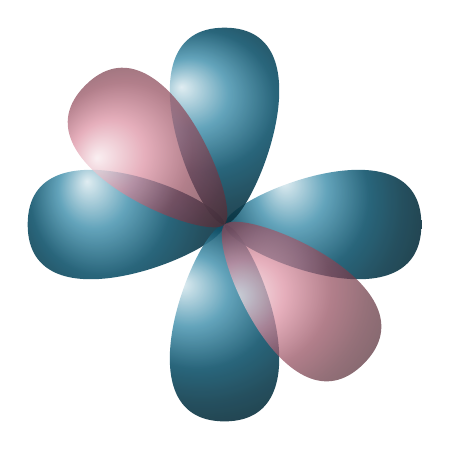
\begin{tikzpicture}[declare function={d=2.5cm;r=.55*d;h=.125*d;R=.85*d;}]
		\tikzstyle{linestyle} = [->,>=stealth,line width=.02*d,\maunhan!80]
		\tikzstyle{myshapestyle} = [ball color = \maudam!90,opacity=.90]
		\path[myshapestyle] (-d,0)..controls +(90:r) and +(90:{.25*r})..(0,0)--
		(0,0)..controls +(-90:{.25*r}) and +(-90:r)..(-d,0);
		\path[myshapestyle] (d,0)..controls +(90:r) and +(90:{.25*r})..(0,0)--
		(0,0)..controls +(-90:{.25*r}) and +(-90:r)..(d,0);
		\path[myshapestyle] (0*R,0*d)..controls +(0:{.25*r}) and +(0:r)..(0*R,d)--
		(0*R,d)..controls +(180:r) and +(180:{.25*r})..(0*R,0);
		\path[myshapestyle] (0*R,-d)..controls +(180:r) and +(180:{.25*r})..(0*R,0*d)--
		(0*R,0*d)..controls +(0:{.25*r}) and +(0:r)..(0*R,-d);
		\begin{scope}[transform canvas={rotate=45}]
			\path[ball color = \maunhan!70,opacity=.7] (0*R,0*d)..controls +(0:{.25*r}) and +(0:r)..(0*R,d)--
			(0*R,d)..controls +(180:r) and +(180:{.25*r})..(0*R,0);
			\path[ball color = \maunhan!70,opacity=.7] (0*R,-d)..controls +(180:r) and +(180:{.25*r})..(0*R,0*d)--
			(0*R,0*d)..controls +(0:{.25*r}) and +(0:r)..(0*R,-d);
		\end{scope}
\end{tikzpicture}}



%
%\begin{tikzpicture}[node distance=.5cm and .5cm]
%			\node (AOx) {\baAOP};
%			\node [right=of AOx](plus) {\color{\maunhan}\LARGE\bfseries\sffamily +};
%			\node [right=of plus] (AOy) {\baAOP};
%			\node[right=of AOy](muiten){\tikz{\path[draw,->,-latex,line width=3pt,\maunhan!80] (0,0)--(3,0);}};
%			\node [right=of muiten] (AOXENPHU){%
%				\begin{tikzpicture}[declare function={d=2.5cm;r=.55*d;h=.125*d;R=.85*d;}]
%					\tikzstyle{linestyle} = [->,>=stealth,line width=.02*d,\maunhan!80]
%					\tikzstyle{myshapestyle} = [ball color = \maudam!90,opacity=.90]
%						\draw[line width=.02*d,\maunhan!80] ({-d - h},0)--({2.8*d + h},0);
%						\draw[line width=.02*d,\maunhan!80] (0*R,{-d - h})--(0*R,{d + h});
%						%% =======================2AO Xen phu truc P-P===========================%%%
%				        \path[myshapestyle] (-d,0)..controls +(90:r) and +(90:{.25*r})..(0,0)--
%				     	(0,0)..controls +(-90:{.25*r}) and +(-90:r)..(-d,0);
%				     	\path[myshapestyle] (d,0)..controls +(90:r) and +(90:{.25*r})..(0,0)--
%				     	(0,0)..controls +(-90:{.25*r}) and +(-90:r)..(d,0);
%				       	\path[myshapestyle] (.8*d,0)..controls +(90:r) and +(90:{.25*r})..(1.8*d,0)--
%				       	(1.8*d,0)..controls +(-90:{.25*r}) and +(-90:r)..(.8*d,0);
%				       	\path[myshapestyle] (2.8*d,0)..controls +(90:r) and +(90:{.25*r})..(1.8*d,0)--
%				       	(1.8*d,0)..controls +(-90:{.25*r}) and +(-90:r)..(2.8*d,0);		
%				         %%%========================Độ Xen phu ben============================%%%
%						\path[myshapestyle] ([shift={(.49cm,-.085cm)}]0,1*d)..controls +(-30:.49*d) and +(-150:.49*d)..([shift={(-.49cm,-.085cm)}]1.8*d,1*d)--
%						(1.8*d,d)..controls +(180:r) and +(180:{.25*r})..(1.8*d,0)--
%						(1.8*d,0*d)..controls +(135:.82*d) and +(45:.82*d)..(0,0*d)--
%						(0*R,0*d)..controls +(0:{.25*r}) and +(0:r)..(0*R,d)--cycle;
%						\begin{scope}[transform canvas={yscale=-1}]
%								\path[myshapestyle] ([shift={(.49cm,-.085cm)}]0,1*d)..controls +(-30:.49*d) and +(-150:.49*d)..([shift={(-.49cm,-.085cm)}]1.8*d,1*d)--
%								(1.8*d,d)..controls +(180:r) and +(180:{.25*r})..(1.8*d,0)--
%								(1.8*d,0*d)..controls +(135:.82*d) and +(45:.82*d)..(0,0*d)--
%								(0*R,0*d)..controls +(0:{.25*r}) and +(0:r)..(0*R,d)--cycle;
%							\end{scope}
%						%%================2 AO xen phủ bên 1======================%%
%						\path[myshapestyle] (0*R,0*d)..controls +(0:{.25*r}) and +(0:r)..(0*R,d)--
%						(0*R,d)..controls +(180:r) and +(180:{.25*r})..(0*R,0);
%						\path[myshapestyle] (0*R,-d)..controls +(180:r) and +(180:{.25*r})..(0*R,0*d)--
%						(0*R,0*d)..controls +(0:{.25*r}) and +(0:r)..(0*R,-d);
%						\draw[line width=.02*d,\maunhan!80] (1.8*d,{-d - h})--(1.8*d,{d + h});
%						\path[myshapestyle] (1.8*d,0*d)..controls +(0:{.25*r}) and +(0:r)..(1.8*d,d)--
%						(1.8*d,d)..controls +(180:r) and +(180:{.25*r})..(1.8*d,0);
%						\path[myshapestyle] (1.8*d,-d)..controls +(180:r) and +(180:{.25*r})..(1.8*d,0*d)--
%						(1.8*d,0*d)..controls +(0:{.25*r}) and +(0:r)..(1.8*d,-d);
%						
%						\begin{scope}[transform canvas={yscale=1.3}]
%								\path[ball color = \maunhan!70,opacity=.5] ([shift={(120:.9112*d)}]0,0*d)..controls +(-30:.8*d) and +(-135:.49*d)..([shift={(135:d)}]1.8*d,0*d)--
%								([shift={(135:d)}]1.8*d,0)..controls +(-135:.9*r) and +(135:{.4*r})..(1.8*d,0)--
%								(1.8*d,0*d)..controls +(135:.05*d) and +(45:.6*d)..(0,0*d)--
%								(0,0)..controls +(45:{.25*r}) and +(-45:r)..([shift={(135:d)}]0,0*d)--cycle;
%								
%								\begin{scope}[transform canvas={yscale=-1,xscale=-1,xshift=-1.8*d}]
%										\path[ball color = \maunhan!70,opacity=.5] ([shift={(120:.9112*d)}]0,0*d)..controls +(-30:.8*d) and +(-135:.49*d)..([shift={(135:d)}]1.8*d,0*d)--
%										([shift={(135:d)}]1.8*d,0)..controls +(-135:.9*r) and +(135:{.4*r})..(1.8*d,0)--
%										(1.8*d,0*d)..controls +(135:.05*d) and +(45:.6*d)..(0,0*d)--
%										(0,0)..controls +(45:{.25*r}) and +(-45:r)..([shift={(135:d)}]0,0*d)--cycle;
%									\end{scope}
%								%%================2 AO xen phủ bên 2======================%%
%								\begin{scope}[transform canvas={rotate=45}]
%										\path[ball color = \maunhan!70,opacity=1] (0*R,0*d)..controls +(0:{.25*r}) and +(0:r)..(0*R,d)--
%										(0*R,d)..controls +(180:r) and +(180:{.25*r})..(0*R,0);
%										\path[ball color = \maunhan!70,opacity=1] (0*R,-d)..controls +(180:r) and +(180:{.25*r})..(0*R,0*d)--
%										(0*R,0*d)..controls +(0:{.25*r}) and +(0:r)..(0*R,-d);
%									\end{scope}
%								\begin{scope}[transform canvas={xshift=1.8*d,rotate=45}]
%										\path[ball color = \maunhan!70,opacity=1] (0*R,0*d)..controls +(0:{.25*r}) and +(0:r)..(0*R,d)--
%										(0*R,d)..controls +(180:r) and +(180:{.25*r})..(0*R,0);
%										\path[ball color = \maunhan!70,opacity=1] (0*R,-d)..controls +(180:r) and +(180:{.25*r})..(0*R,0*d)--
%										(0*R,0*d)..controls +(0:{.25*r}) and +(0:r)..(0*R,-d);
%									\end{scope}
%							\end{scope}
%				\end{tikzpicture}
%			};
%			\node[below=of AOx,yshift=-.2cm]{\color{\maunhan}\LARGE\bfseries\sffamily N};
%			\node[below=of AOy,yshift=-.2cm]{\color{\maunhan}\LARGE\bfseries\sffamily N};
%			\node[below=of AOXENPHU,yshift=.15cm]{\color{\maunhan}\LARGE\bfseries\sffamily phân tử N$\mathbf{_2}$};
%			\node[above=of AOXENPHU,yshift=-2.5cm]{\color{white}\Huge $\mathbf{\pi}$};
%			\node[below=of AOXENPHU,yshift=3.7cm]{\color{white}\Huge $\mathbf{\sigma}$};
%\end{tikzpicture}



























\end{document}